\documentclass[a4paper]{article}
\usepackage{times}
\usepackage[utf8]{inputenc}
\usepackage{selinput}
\usepackage{upquote}
\usepackage[margin=2cm, rmargin=4cm, tmargin=3cm]{geometry}
\usepackage{tcolorbox}
\usepackage{xspace}
\usepackage[french]{babel}
\usepackage{url}
\usepackage{hyperref}
\usepackage{fontawesome5}
\usepackage{marginnote}
\usepackage{ulem}
\usepackage{tcolorbox}
\usepackage{graphicx}
%\usepackage[top=Bcm, bottom=Hcm, outer=Ccm, inner=Acm, heightrounded, marginparwidth=Ecm, marginparsep=Dcm]{geometry}


\newtcolorbox{Example}[1]{colback=white,left=20pt,colframe=slideblue,fonttitle=\bfseries,title=#1}
\newtcolorbox{Solutions}[1]{colback=white,left=20pt,colframe=green,fonttitle=\bfseries,title=#1}
\newtcolorbox{Conseils}[1]{colback=white,left=20pt,colframe=slideblue,fonttitle=\bfseries,title=#1}
\newtcolorbox{Warning}[1]{colback=white,left=20pt,colframe=warning,fonttitle=\bfseries,title=#1}

\setlength\parindent{0pt}

  %Exercice environment
  \newcounter{exercice}
  \newenvironment{Exercice}[1][]
  {
  \par
  \stepcounter{exercice}\textbf{Question \arabic{exercice}:} (\faClock \enskip \textit{#1})
  }
  {\bigskip}
  

% Title
\newcommand{\titre}{\begin{center}
  \section*{Algorithmes et Pensée Computationnelle}
\end{center}}
\newcommand{\cours}[1]
{\begin{center} 
  \textit{#1}\\
\end{center}
  }


\newcommand{\exemple}[1]{\newline~\textbf{Exemple :} #1}
%\newcommand{\attention}[1]{\newline\faExclamationTriangle~\textbf{Attention :} #1}

% Documentation url (escape \# in the TP document)
\newcommand{\documentation}[1]{\faBookOpen~Documentation : \href{#1}{#1}}

% Clef API
\newcommand{\apikey}[1]{\faKey~Clé API : \lstinline{#1}}
\newcommand{\apiendpoint}[1]{\faGlobe~Url de base de l'API \href{#1}{#1}}

%Listing Python style
\usepackage{color}
\definecolor{slideblue}{RGB}{33,131,189}
\definecolor{green}{RGB}{0,190,100}
\definecolor{blue}{RGB}{121,142,213}
\definecolor{grey}{RGB}{120,120,120}
\definecolor{warning}{RGB}{235,186,1}

\usepackage{listings}
\lstdefinelanguage{texte}{
    keywordstyle=\color{black},
    numbers=none,
    frame=none,
    literate=
           {é}{{\'e}}1
           {è}{{\`e}}1
           {ê}{{\^e}}1
           {à}{{\`a}}1
           {â}{{\^a}}1
           {ù}{{\`u}}1
           {ü}{{\"u}}1
           {î}{{\^i}}1
           {ï}{{\"i}}1
           {ë}{{\"e}}1
           {Ç}{{\,C}}1
           {ç}{{\,c}}1,
    columns=fullflexible,keepspaces,
	breaklines=true,
	breakatwhitespace=true,
}
\lstset{
    language=Python,
	basicstyle=\bfseries\footnotesize,
	breaklines=true,
	breakatwhitespace=true,
	commentstyle=\color{grey},
	stringstyle=\color{slideblue},
  keywordstyle=\color{slideblue},
	morekeywords={with, as, True, False, Float, join, None, main, argparse, self, sort, __eq__, __add__, __ne__, __radd__, __del__, __ge__, __gt__, split, os, endswith, is_file, scandir, @classmethod},
	deletekeywords={id},
	showspaces=false,
	showstringspaces=false,
	columns=fullflexible,keepspaces,
	literate=
           {é}{{\'e}}1
           {è}{{\`e}}1
           {ê}{{\^e}}1
           {à}{{\`a}}1
           {â}{{\^a}}1
           {ù}{{\`u}}1
           {ü}{{\"u}}1
           {î}{{\^i}}1
           {ï}{{\"i}}1
           {ë}{{\"e}}1
           {Ç}{{\,C}}1
           {ç}{{\,c}}1,
    numbers=left,
}

\newtcbox{\mybox}{nobeforeafter,colframe=white,colback=slideblue,boxrule=0.5pt,arc=1.5pt, boxsep=0pt,left=2pt,right=2pt,top=2pt,bottom=2pt,tcbox raise base}
\newcommand{\projet}{\mybox{\textcolor{white}{\small projet}}\xspace}
\newcommand{\optionnel}{\mybox{\textcolor{white}{\small Optionnel}}\xspace}
\newcommand{\advanced}{\mybox{\textcolor{white}{\small Pour aller plus loin}}\xspace}
\newcommand{\auto}{\mybox{\textcolor{white}{\small Auto-évaluation}}\xspace}


\usepackage{environ}
\newif\ifShowSolution
\NewEnviron{solution}{
  \ifShowSolution
	\begin{Solutions}{\faTerminal \enskip Solution}
		\BODY
	\end{Solutions}
  \fi}


  \usepackage{environ}
  \newif\ifShowConseil
  \NewEnviron{conseil}{
    \ifShowConseil
    \begin{Conseils}{\faLightbulb \quad Conseil}
      \BODY
    \end{Conseils}

    \fi}

    \usepackage{environ}
  \newif\ifShowWarning
  \NewEnviron{attention}{
    \ifShowWarning
    \begin{Warning}{\faExclamationTriangle \quad Attention}
      \BODY
    \end{Warning}

    \fi}
  

%\newcommand{\Conseil}[1]{\ifShowIndice\ \newline\faLightbulb[regular]~#1\fi}



\usepackage{listings}
\usepackage{array}
\newcolumntype{C}[1]{>{\centering\let\newline\\\arraybackslash\hspace{0pt}}m{#1}}

\begin{document}

% Change the following values to true to show the solutions or/and the hints
\ShowSolutionfalse
\ShowConseiltrue
\titre
\cours{Programmation de base - Exercices de base}

Le but de cette séance est d'aborder des notions de base en programmation. Au terme de cette séance, l'étudiant sera capable de: \\

\begin{itemize}
	\item Définir une variable, définir son type et sa valeur.
	\item Définir une fonction et comprendre son rôle.
	\item Utiliser des notions d'algèbre booléenne.
	\item Comprendre la notion d'entrée/sortie. \\
\end{itemize} 

Les langages qui seront utilisés pour cette séance sont Java et Python. Assurez-vous d'avoir bien installé Intellij. Si vous rencontrez des difficultés, n'hésitez pas à vous référer au guide suivant: \href{https://moodle.unil.ch/pluginfile.php/1721328/mod_resource/content/3/prerequisite.pdf}{tutoriel d'installation des outils et prise en main de l'environnement de travail}.\\

\section{Représentation de nombres entiers}

\begin{Exercice}[5 minutes] \textbf{Entiers non signés}
	Sur 8 bits convertir 113$_{(10)}$ en base binaire.
   
    \begin{conseil}
		Faire un tableau comme présenté dans la diapositive 10 du cours de la semaine 3. Essayer de décomposer le nombre en une somme de puissances de 2.
    \end{conseil}
    
    \begin{solution}
        Méthode 1: Utiliser la division par 2 comme vu dans la première séance d'exercices\\
        
        Méthode 2 : Utiliser les puissances de 2 pour décomposer le nombre (vu également dans la première séance d'exercices).
        
        113 = 64 + 32 + 16 + 1 = 1 * $2^6$ + 1 * $2^5$ + 1* $2^4$ + 1 * $2^0$ \\
        
        \begin{tabular}{| p{1cm} | p{1cm} | p{1cm} | p{1cm} | p{1cm} | p{1cm} | p{1cm} | p{1cm} | p{1cm} |} 
            \hline
	      	$2^7$ & $2^6$ & $2^5$ & $2^4$ & $2^3$ & $2^2$ & $2^1$ & $2^0$ \\ [0.5ex]
	    	\hline
            128 & 64 & 32 & 16 & 8 & 4 & 2 & 1 \\ [0.5ex] 
            \hline
            0 & 1 & 1 & 1 & 0 & 0 & 0 & 1 \\ [0.5ex] 
            \hline
        \end{tabular} \\
        
        On obtient donc 01110001$_{(2)}$ \\
    \end{solution}
\end{Exercice}

\begin{Exercice}[5 minutes] \textbf{Entiers signés négatifs}\\
    En utilisant le résultat de la question précédente, convertir sur 8 bits -113$_{(10)}$ en base binaire. \\

    \begin{conseil}
        \begin{itemize}
        	\item Il faut prendre la représentation sur 7 bits d'un nombre entier non signé.
        	\item On rajoute un 8ème bit qui sera le signe.
        	\item Pour cet exercice, reprendre l'expression non signée de la question précédente (question 1 - Entiers non signés) et changer le premier bit en conséquence.
        	\item Le premier bit vaut 0 pour un nombre positif et 1 pour un nombre négatif.
        \end{itemize} 
    \end{conseil}
    
    \begin{solution}
         113$_{(10)}$ = 01110001$_{(2)}$ \\
         
         En changeant le premier bit à 1 pour faire passer le nombre en nombre négatif on obtient : \\
         
         -113$_{(10)}$ = 11110001$_{(2)}$ \\
    \end{solution}
\end{Exercice}

\begin{Exercice}[5 minutes] \textbf{Complément à 1}\\
    Ecrire le complément à 1 de -113$_{(10)}$ . \\

	Quelle est la différence entre cette méthode et la précédente ? \\

    \begin{conseil}
        \begin{itemize}
        	\item En programmation l'opposé d'une variable est \lstinline{not}(la variable). Ici, le même principe s'applique. L'opposé de 0 en binaire est 1.
        	\item Pour étudier la différence, il faut regarder les différentes manières d'exprimer -0 en binaire (se référer à la diapositive 11 du cours de la semaine 3).
        \end{itemize} 
    \end{conseil}
    
    \begin{solution}
    	113$_{(10)}$ = 01110001$_{(2)}$ \\
    	
        \begin{tabular}{| p{1cm} | p{1cm} | p{1cm} | p{1cm} | p{1cm} | p{1cm} | p{1cm} | p{1cm} | p{1cm} |} 
            \hline
            0 & 1 & 1 & 1 & 0 & 0 & 0 & 1 \\ [0.5ex] 
            \hline
            not & not & not & not & not & not & not & not \\ [0.5ex]
            \hline
            1 & 0 & 0 & 0 & 1 & 1 & 1 & 0 \\ [0.5ex]
            \hline
        \end{tabular} \\
        
        avec cette méthode, -113$_{(10)}$ = 10001110$_{(2)}$ \\
        
        L'intervalle de cette méthode ne change pas par rapport à la précédente. Par contre, l'expression de -0 sera différente.\\
        
        Signé: -0$_{(10)}$ = 10000000$_{(2)}$ \\
        
        Complément à 1: -0$_{(10)}$ = 11111111$_{(2)}$ \\
        
        Les deux ont le même intervalle: [-127$_{(10)}$,+127$_{(10)}$] \\
        
    \end{solution}
\end{Exercice}

\begin{Exercice}[5 minutes] \textbf{Complément à 2}\\
    Quel est le complément à 2 de -113$_{(10)}$ et quelle est l'utilité de cette représentation ? \\

    \begin{conseil}
    
    Exemple du cours avec 87$_{(10)}$ \\
    
    87$_{(10)}$ = 01010111$_{(2)}$ \\
    
         \begin{tabular}{| p{1cm} | p{1cm} | p{1cm} | p{1cm} | p{1cm} | p{1cm} | p{1cm} | p{1cm} | p{1cm} |} 
            \hline
            a & 0 & 1 & 0 & 1 & 0 & 1 & 1 & 1 \\ [0.5ex] 
            \hline
            b & 1 & 0 & 1 & 0 & 1 & 0 & 0 & 0 \\ [0.5ex]
            \hline
            c & 1 & 0 & 1 & 0 & 1 & 0 & 0 & 1 \\ [0.5ex]
            \hline
        \end{tabular} \\
        
        a : convertir le nombre en binaire \\
        
        b : inverser tous les bits \\
        
        c : rajouter 1 au nombre pour obtenir le complément à 2 \\
        
        On obtient donc -87$_{(10)}$ = 10101001$_{(2)}$ \\
    \end{conseil}
    
    \begin{solution}
    	Ici, il suffit donc d'ajouter 1 au complément à 1 de -113$_{(10)}$ \\
    	
    	On obtient donc 10001111$_{(2)}$ \\
    	
    	Concernant l'intervalle, il est changé, étant donné qu'il n'existe plus qu'une seule représentation possible pour -0$_{(10)}$. \\
    	
    	Le nouvel intervalle est donc [-128$_{(10)}$,+127$_{(10)}$]
        
    \end{solution}
\end{Exercice}

\begin{Exercice}[10 minutes] \textbf{Floating point}\\
    
    Voici la représentation en binaire d'un nombre à virgule flottante: \\
    
     \begin{tabular}{| p{1cm} | p{3cm} | p{9.5cm} | p{1cm} | p{1cm} | p{1cm} | p{1cm} | p{1cm} | p{1cm} |} 
            \hline
            signe & exposant & mantisse \\ [0.5ex] 
            \hline
            0 & 10110101 & 01000001000000000000001 \\ [0.5ex]
            \hline
	\end{tabular}
	
    Que vaut cette représentation en base 10 ? Utiliser la représentation des floating point (avec un biais de 127) Arrondir les résultats intermédiaires et la valeur finale au 3ème chiffre significatif après la virgule. \\
	
    \begin{conseil}
    
    \begin{itemize}
    	\item Se référer à la diapositive 15 du cours de la semaine 3 pour plus de détails.
    	\item Poser chaque calcul, et ensuite tout fusionner avec la formule.
    	\item L'exposant et la mantisse sont des entiers positifs, donc non signés.
    \end{itemize}
    
    \end{conseil}
    
    \begin{solution}
        \begin{itemize}
        	\item Signe du nombre : $(-1)^{signe}$ = $(-1)^0$ = 1
        	\item Exposant en base 10 : 10110101$_{(2)}$ = 181$_{(10)}$
        	\item Pour obtenir l'exposant, il faut encore lui appliquer le biais, il faut soustraire 127 à notre résultat. Ici on aura $2^{(181-127)}$ = $2^{54}$
        	\item Mantisse : 01000001000000000000001$_{(2)}$ = 1 + 1*$2^{-2}$ + 1*$2^{-8}$ + 1*$2^{-23}$ = 1.254$_{(10)}$
        	\item Valeur = Signe * Mantisse * $2^{exposant-127}$ = 1 * 1.254 * $2^{54}$ = 2.259 * $10^{16}$
        \end{itemize}
    \end{solution}
\end{Exercice}
\newpage

\newpage

\section{Typage}

Le but de cette partie des travaux pratiques est de comprendre les notions de typage statique et dynamique, ainsi que leur impact sur l’exécution et la gestion des erreurs. \\

\begin{Exercice}[3 minutes]  \textbf{Les types de variables}\\
    
    Quelles sont les principaux types de variable (donnez en 3), comment les déclareriez vous en Python et en Java ? \\

    \begin{conseil}
    
        Se référer aux diapositives du cours ou à la documentation officielle de votre langage de programmation préféré.
        
    \end{conseil}
    \begin{solution}
    
        Les principaux types de variables sont les suivants : Integer (int), Float, String (str), Boolean (bool).\\

		En Python :    
        
    	\lstinputlisting{resources/solutions/Question6.py} 
    	
    	
    	En Java : 
    	
    	\lstinputlisting{resources/solutions/Question6.java} 
    	
    	Il existe d'autres types de variable, comme par exemple les double.
 
    \end{solution}
\end{Exercice}


\begin{Exercice}[5 minutes]  \textbf{Typage statique et dynamique}\\
    
    Parmi ces différents programmes, lesquels pourront être exécutés sans problème et lesquels lèveront des erreurs? Dans le cas où ils génèreraient des erreurs, expliquez la raison de ces erreurs.\\
    
    \textbf{Java :}
    
    \lstinputlisting{resources/Question7.java} 
    
    \textbf{Python :}
    
    \lstinputlisting{resources/Question7.py} 
    

    \begin{conseil}
    
        En Java, le type est statique, ce qui signifie qu'à partir du moment où vous créez une variable, un type va lui être attribué (par vous ou par le code en lui-même par déduction). Ce type ne pourra pas être changé, et si vous tentez de le faire (en lui attribuant une valeur d'un autre type par exemple), une erreur sera levée. \\

En Python, le typage est dynamique, il est donc tout à fait possible de changer le type d'une variable sans déclencher d'erreur. \\

    \end{conseil}

    \begin{Example}{\faExclamationTriangle \quad Erreurs fréquentes}
        Au cas où vous exécuteriez les programmes 2, 4 et 5 et rencontriez l'erreur suivante: \lstinline{Exception in thread "main" java.lang.UnsupportedClassVersionError: ... has been compiled by a more recent version of the Java Runtime (class file version 54.0), this version of the Java Runtime only recognizes class file versions up to 52.0}, suivez les étapes ci-dessous:
        \begin{enumerate}
            \item Mettez à jour votre JDK en téléchargeant la version adéquate via le lien suivant: \url{https://www.oracle.com/java/technologies/javase-jdk15-downloads.html}.
            \item Une fois votre JDK installé, redémarrez IntelliJ
            \item Dans la barre de menus, cliquez sur \textbf{Run $>$ Edit Configurations}.
            \item Dans la fenêtre qui apparaitra (capture ci-dessous), sélectionnez la version du JRE la plus récente.
        \end{enumerate}
        
    \end{Example}
    \begin{figure}[h]
        \centering
        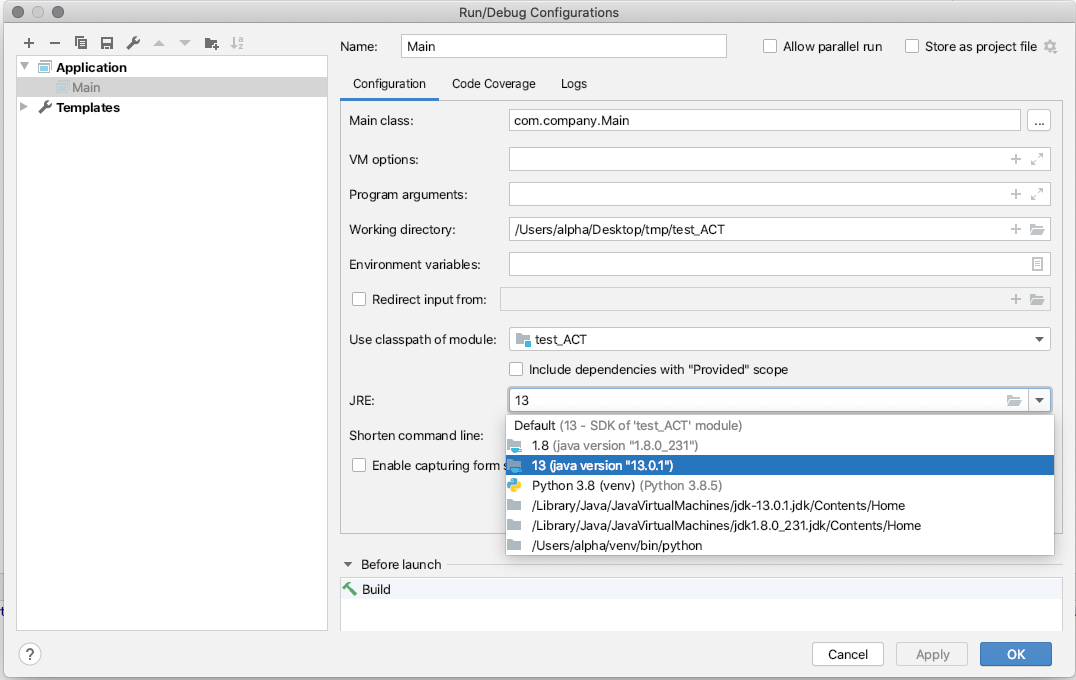
\includegraphics[width=1\textwidth]{resources/jre.png}
        \caption{Fenêtre de configuration de l'environnement de développement Java.}
    \end{figure}
    \begin{solution}

        \textbf{En Java}        
        \begin{itemize}
        	\item Programme 1 : OK
        	\item Programme 2 : Ce code ne fonctionnera pas car on essaye de changer le type de la variable\_2, ce qui est impossible avec un typage statique comme en java. Ici le type de la variable est ``déduit'' lors de l'exécution du programme.
        	\item Programme 3 : Tout comme le programme précédent, ce code ne fonctionnera pas car on essaye de changer le type de la variable\_2, ce qui est impossible avec un typage statique comme en java.
        	\item Programme 4 : Ce code ne fonctionnera pas car on essaye de changer le type de la variable\_1, ce qui est impossible avec un typage statique comme en java. Ici le type de la variable est ``déduit'' lors de l'exécution du programme.
        	\item Programme 5 : OK
        	\item Programme 6 : Ce code ne fonctionnera pas car on essaye de changer le type de la variable\_1, ce qui est impossible avec un typage statique comme en java. \\
        \end{itemize}
        
        \textbf{En Python}
        
        \begin{itemize}
        	\item Programme 7 : OK
        	\item Programme 8 : OK
        \end{itemize}
        
        
    \end{solution}
\end{Exercice}

\begin{Exercice}[5 minutes] \textbf{Détection d'erreurs}

    Soient les deux programmes suivants, l’un en Java et l’autre en Python. Chaque programme comporte une fonction nommée \lstinline{raise_error()} levant une exception de type \lstinline{TypeError}. Dans les deux cas, cette fonction ne sera pas appelée lors de l'exécution (la condition est remplie d’office). Pourtant, l’un de ces deux codes lèvera une erreur, et l’autre sera exécuté sans problème. Quel code lèvera l’erreur et lequel sera exécuté ? Justifiez votre réponse.\\\\
    \textbf{En Java:}
    
    \lstinputlisting{resources/Question8.java}
    
    \textbf{En Python:}
    \lstinputlisting{resources/Question8.py}  
    
    
    \begin{conseil}
        Pensez à vérifier le type des variables. Faites attention à la différence principale entre le typage des variables en Java et le typage en Python.
    \end{conseil}
    \begin{solution}
    	Le premier code va lever une erreur de type \lstinline{Type error}, même si la fonction n'est jamais appelée. En Java, le typage est statique, et de ce fait, toutes les erreurs seront détectées avant exécution du programme.

Le deuxième code en revanche ne va pas lever d'erreur. En python, le typage est dynamique et de ce fait, l'erreur ne sera détectée qu'au moment ou le programme sera exécuté. Si on change le \lstinline{True} en \lstinline{False}, la fonction provoquant l'erreur va être appelée, et dans ce cas ci, l'erreur sera mise en évidence.\\
    \end{solution}

\end{Exercice}
\newpage

\section{Bases en programmation}
Le but de cette section est d'écrire vos premières lignes de code. Les notions abordées concerneront les variables, les fonctions, et les interactions avec l'utilisateur (input/output). Vous pouvez les écrire en Java ou en Python.\\

\begin{Exercice}[5 minutes] \textbf{Output (Java ou Python)}\\
   Créez une variable \textit{nom} (str) contenant votre nom, et une autre \textit{prenom} (str) contenant votre prénom puis affichez : "Bonjour, \textit{prenom nom}". \\
   
    \begin{conseil}
        Utilisez la fonction \lstinline{print()} de Python et \lstinline{System.out.println()} de Java. 
        
    \end{conseil}
    \begin{solution}
    
    \textbf{Python:} 
    \lstinputlisting{resources/solutions/Question9.py}
    
    \textbf{\\Java:} 
    \lstinputlisting{resources/solutions/Question9.java}  
       
        
    \end{solution}   
\end{Exercice}

\begin{Exercice}[5 minutes] \textbf{Input (Java ou Python)}\\
   En vous référant à l'exercice précédent (\textbf{Output (Java ou Python)}), demandez à l'utilisateur d'entrer son nom et son prénom via la fonction \lstinline{input()} au lieu d'initialiser vous-même les variables. \\
   
    \begin{conseil}
       Utilisez la fonction \lstinline{input()} en Python, la classe \lstinline{Scanner()} en Java (n'oubliez pas d'ajouter \lstinline{import java.util.Scanner;}) tout au début de votre code. 
        
    \end{conseil}
    \begin{solution}
    
    \textbf{Python:} 
    \lstinputlisting{resources/solutions/Question10.py}
    
    \textbf{\\Java:}
    \lstinputlisting{resources/solutions/Question10.java}  
       
        
    \end{solution}   
\end{Exercice}

\begin{Exercice}[5 minutes] \textbf{Format d'impression (Python uniquement)}\\
   Créez et assignez des valeurs à 2 variables \textit{prenom} (str) et \textit{age} (int), puis affichez: "Je m'appelle \textit{prenom} et j'ai \textit{age} ans". Gérez le format de l'impression via l'opérateur +, puis en utilisant la fonction \lstinline{format()}. \\
   
    \begin{conseil}
       N'hésitez pas à consulter ce lien pour plus de détails concernant l'utilisation de la fonction format(): \url{
        https://docs.python.org/fr/3.5/library/stdtypes.html\#str.format}
    \end{conseil}
    \begin{solution}
     
    \lstinputlisting{resources/solutions/Question11.py}
           
    \end{solution}   
\end{Exercice}

\begin{Exercice}[3 minutes] \textbf{Type (Python uniquement)}\\
   Déclarez deux variables \textit{nom} (String) et \textit{age} (int), puis affichez le type de chacune de ces deux variables.
   
    \begin{conseil}
       Vous pouvez contrôler le type de vos variables via la fonction \lstinline{type()}.
        
    \end{conseil}
    \begin{solution}
     
    \lstinputlisting{resources/solutions/Question12.py}
           
    \end{solution}   
\end{Exercice}

\begin{Exercice}[5 minutes] \textbf{Conversion des variables (Type casting) (Java ou Python)}\\
   Il est possible de convertir une variable d'un certain type vers un autre type. Il est par exemple possible de changer un \lstinline{int} en \lstinline{float} ou un \lstinline{float} en \lstinline{int}. Cette opération se nomme le \textit{Type Casting}. \\
   Déclarez une variable \textit{nombre\_entier} de type \lstinline{int}, puis une autre variable \textit{nombre\_decimal} de type \lstinline{float}. Affichez \textit{nombre\_entier} en le convertissant en \lstinline{float} et \textit{nombre\_decimal} en le convertissant en \lstinline{int}. \\
   
    \begin{conseil}
       Utilisez la fonction \lstinline{int(float)} et \lstinline{float(int)} en Python / Utilisez \lstinline{(int) float} et (float) int en Java.
        
    \end{conseil}
    \begin{solution}
    
    \textbf{Python:}
    
    \lstinputlisting{resources/solutions/Question13.py}
    
    \textbf{\\Java:}
    \lstinputlisting{resources/solutions/Question13.java}
           
    \end{solution}   
\end{Exercice}

\begin{Exercice}[3 minutes] \textbf{Calculs (multiplication) (Java ou Python)}\\

   Créez 2 variables \textit{facteur\_1} (= 11) et \textit{facteur\_2} (= 3). Multipliez la première variable par la deuxième et stockez le résultat dans une nouvelle variable \textit{produit}. Vous pouvez afficher les différentes variables pour voir leurs valeurs. Vous pouvez répéter l'exercice avec l'addition et la soustraction. \\
   
    \begin{conseil}
      	L'opérateur de multiplication est le *, celui d'addition est le + et celui de soustraction est le -.
        
    \end{conseil}
    \begin{solution}
    
    \textbf{Python:}
    \lstinputlisting{resources/solutions/Question14.py}
    
    \textbf{\\Java:}
    \lstinputlisting{resources/solutions/Question14.java}
           
    \end{solution}   
\end{Exercice}

\begin{Exercice}[10 minutes] \textbf{Calculs (division) (Java ou Python)}\\
    Créez 2 variables \textit{nb\_bonbons} avec pour valeur 11 et \textit{nb\_personnes} avec pour valeur 3. Divisez la première variable par la deuxième et stockez le résultat dans une nouvelle variable \textit{bonbons\_personnes}. Pour finir, calculez le nombre de bonbons restants via l'opérateur \% (modulo) et stockez le résultat dans une nouvelle variable \textit{reste}. Vous pouvez afficher les différentes variables pour voir leurs valeurs. \\
    
     \begin{conseil}
           Attention, en Python il existe 2 opérateurs de division, / effectue une division classique, tandis que // effectue une division entière. En Java, si vous travaillez uniquement avec des int, / effectuera une division entière tandis que si vous travaillez avec au moins un float, / effectuera une division classique. Vous pouvez aussi formater le type du résultat lorsque vous créez une variable.
         
     \end{conseil}
     \begin{solution}
     
     \textbf{Python:}
     
     \lstinputlisting{resources/solutions/Question15.py}
     
     \textbf{\\Java:}
     \lstinputlisting{resources/solutions/Question15.java}
            
     \end{solution}   
 \end{Exercice}
 
\begin{Exercice}[5 minutes] \textbf{Calculs (incrémentation / décrémentation) (Java ou Python)}\\
   Gardez vos variables de l'exercice précédent (\textbf{Calculs (division) (Java ou Python)}), augmentez la valeur de \textit{nb\_bonbons} de 1, et diminuez celle de \textit{nb\_personnes} de 1.  \\
   
    \begin{conseil}
      	Vous pouvez utiliser les opérateurs += et -= en Python, et les opérateurs ++ et \textit{- -} en Java.
        
    \end{conseil}
    \begin{solution}
    
    \textbf{Python:}
    \lstinputlisting{resources/solutions/Question16.py}
    
    \textbf{\\Java:}
    \lstinputlisting{resources/solutions/Question16.java}
           
    \end{solution}   
\end{Exercice}

\begin{Exercice}[5 minutes] \textbf{Manipulation des chaînes de caractères (indexation) (Java ou Python)}\\
   Créez une variable \textit{mon\_mot} de type chaîne de caractères avec pour valeur \textbf{``Hard But Cool !!''}. Créez ensuite une variable \textit{premiere} contenant la première lettre de \textit{mon\_mot} en utilisant l'indexation. Créez enfin une variable \textit{derniere} contenant la dernière lettre de \textit{mon\_mot} en utilisant l'indexation. Affichez les résultats. Qu'obtenez-vous? \\
   
    \begin{conseil}
      	Pour Python, utilisez \lstinline{[]}, et pour Java, utilisez la fonction \lstinline{substring()} ainsi que la fonction \lstinline{length()} qui permet d'obtenir la taille d'un élément.
        
    \end{conseil}
    \begin{solution}
    
    \textbf{Python:}
    \lstinputlisting{resources/solutions/Question17.py}
    
    \textbf{\\Java:}
    \lstinputlisting{resources/solutions/Question17.java}
           
    \end{solution}   
\end{Exercice}

\begin{Exercice}[5 minutes] \textbf{Manipulation des chaînes de caractères (indexation 2) (Java ou Python)}\\
   Gardez votre variable, \textit{mon\_mot} et créez une variable \textit{lettre\_5} contenant la cinquième lettre de \textit{mon\_mot} en utilisant l'indexation. Créez ensuite une variable \textit{lettre\_9\_13} contenant les lettres 9, 10, 11, 12, 13 de \textit{mon\_mot}. Afficher les résultats et voyez ce que vous obtenez.  \\
   
    \begin{conseil}
      	Attention, ici les espaces comptent comme des lettres ! \\

		Pour Python, utilisez \lstinline{[:]}, et pour Java, utilisez la fonction \lstinline{substring()}.
        
    \end{conseil}
    \begin{solution}
    
    \textbf{Python:}    
    \lstinputlisting{resources/solutions/Question18.py}
    
    \textbf{\\Java:}
    \lstinputlisting{resources/solutions/Question18.java}
           
    \end{solution}   
\end{Exercice}

\begin{Exercice}[5 minutes] \textbf{Les fonctions (fonctions basiques) (Java ou Python))}\\
  Définissez une fonction nommée \lstinline{ping()} qui, lorsqu'elle est appelée, affiche ``pong''. Appelez la plusieurs fois et observez le résultat.  \\
   
    \begin{conseil}
        \begin{itemize}
            \item Référez vous aux diapositives du cours pour la création et l'appel des fonctions. 
            \item Vous pourriez utiliser une boucle for pour effectuer plusieurs appels à la fonction \lstinline{ping()}.
        \end{itemize}        
    \end{conseil}
    \begin{solution}
    
        \textbf{Python}:
        \lstinputlisting{resources/solutions/Question19.py}
        
        \textbf{\\Java}:
        \lstinputlisting{resources/solutions/Question19.java}
           
    \end{solution}   
\end{Exercice}

\begin{comment}
   \begin{Exercice}[5 minutes] \textbf{Les Fonctions (Fonction multiplication) (Java ou Python)}\\
   Définissez une fonction nommée \lstinline{multiplicateur()} qui prend deux arguments \textit{multiple\_1} et \textit{multiple\_2}, les multiplie et retourne le résultat. Stockez le résultat de \lstinline{multiplicateur(2,3)} dans une variable \textit{resultat} et affichez la.   \\
   
    \begin{conseil}
        \begin{itemize}
            \item Référez vous au cours pour la création et l'appel des fonctions.
            \item Pour retourner une valeur au lieu de l'imprimer, utilisez le mot clé \lstinline{return} (pour Python et Java).
        \end{itemize}        
    \end{conseil}
    \begin{solution}
        \textbf{Python}:
        \lstinputlisting{resources/Question23.py}
        
        \textbf{\\Java}:
        \lstinputlisting{resources/Question23.java}
    \end{solution}   
\end{Exercice} 
\end{comment}

\begin{Exercice}[5 minutes] \textbf{Les Fonctions (Fonctions Aire et Périmètre) (Java ou Python)}\\
    Définissez deux fonctions nommées \lstinline{aire()} et \lstinline{perimètre()} qui prennent un argument (\lstinline{rayon}) et renvoient respectivement l'aire et le périmètre d'un cercle. Stockez les résultats dans des variables \lstinline{aire} et \lstinline{perimetre} et affichez le contenu de ces variables.   \\
   
    \begin{conseil}
        \begin{itemize}
            \item Référez vous au cours pour la création et l'appel des fonctions.
            \item Pour retourner une valeur au lieu de l'imprimer, utilisez le mot clé \lstinline{return} (pour Python et Java).
            \item Pour rappel, le périmètre d'un cercle s'obtient en utilisant la formule $P = 2*\pi*r$ et l'aire s'obtient en utilisant la formule $A = r^2*\pi$.
        \end{itemize}        
    \end{conseil}
    \begin{solution}
        \textbf{Python}:
        \lstinputlisting{resources/solutions/Question20.py}
        
        \textbf{\\Java}:
        \lstinputlisting{resources/solutions/Question20.java}
    \end{solution}   
\end{Exercice} 


\newpage
\section{Opérateurs et conditions Booléennes (Python uniquement)}
Le principe d'une valeur booléenne est qu'elle ne puisse contenir que 2 valeurs possibles, soit \lstinline{True}, soit \lstinline{False}. Il est possible de les définir en leur associant une de ces valeurs d'emblée ou de les obtenir en effectuant une comparaison. Pour ce faire, il faut utiliser des opérateurs booléens. Voici les plus utilisés : $==$ (est égal), $!=$ (n'est pas égal), $<$ (est strictement plus petit), $<=$ (est plus petit ou égal), $>$ (est strictement plus grand), $>=$ (est plus grand ou égal). Si la condition est satisfaite, on obtiendra \lstinline{True}, si elle ne l'est pas, on obtiendra \lstinline{False}. L'utilisation de l'opérateur \lstinline{not} inversera le résultat.\\

Dans les exercices suivants, vous devrez anticiper la valeur que la console va vous donner (résultat du(des) print(s)). \\

\begin{conseil}
	Utilisez les tables de vérité présentées à la diapositive 23 du cours.
\end{conseil}


\begin{Exercice}[5 minutes] Qu'affichera le programme suivant?
    
    \lstinputlisting{resources/Question21.py}

    \begin{solution}
        False 
        
        True 
        
        True 
        
        False 
        
        False \\
    \end{solution}
\end{Exercice}
    
\begin{Exercice}[5 minutes] Qu'affichera le programme suivant?
    
    \lstinputlisting{resources/Question22.py}

    \begin{solution}
        True 
        
        False 
        
        True 
        
        True \\
    \end{solution}
    
\end{Exercice}
    
\begin{Exercice}[5 minutes] Qu'affichera le programme suivant?
    
    \lstinputlisting{resources/Question23.py}

    \begin{solution}
        output 1\\
        output 2\\
        output 3
    \end{solution}
    
\end{Exercice}

\newpage
\section{Conditions}
Le but de cette section est de vous entraîner à la lecture de code, la compréhension des opérateurs booléens et au ``case switching'' à travers le branchement conditionnel.
\\
\begin{Exercice}[10 minutes] \textbf{Branchement conditionnel en Java}\\
  Qu'affiche le programme suivant? 
  
  \lstinputlisting{resources/Question24.java}
   
    \begin{conseil}
      	\begin{itemize}
      		\item \lstinline{break} indique que l'on sort de l'accolade. Les cas suivants ne seront pas traités.
      		\item L'absence de \lstinline{break} indique que l'on va rentrer dans tous les cas suivants, jusqu'à enfin atteindre un \lstinline{break}.
      		\item Lorsque l'on pose case n où n est un nombre cela est équivalent au test \lstinline{n == numero_mois}. Ce test est aussi valable si on cherche à comparer des chaînes de caractères (par exemple si \lstinline{numero_mois = "Juin"}, à ce moment là \lstinline{n} sera aussi une chaîne de caractères).\\\\
      	\end{itemize}
        
    \end{conseil}
    \begin{solution}
    
    Juillet
    
	Aout
	
	Décembre \\
	
	Explications : \\
	
	\begin{itemize}
      		\item Comme la case 7 ne contient pas de break et modifie \lstinline{numero_mois}, la lecture du code va continuer.
      		\item On rentre dans le case 9, qui contient un break. Le \lstinline{numero_mois} sera aussi modifié mais cela ne sera pas important car on sort de l'accolade et les cas suivants ne seront pas traités.
      \end{itemize}
           
    \end{solution}   
\end{Exercice}

\begin{Exercice}[5 minutes] \textbf{Conditions en Python}\\
  Qu'affiche le programme suivant?
  \lstinputlisting{resources/Question25.py}
   
    \begin{conseil}
      	\begin{itemize}
      		\item Il faut vérifier la condition de chaque cas de façon linéaire.
      		\item Une fois une condition vérifiée, toutes celles d'après ne sont pas traitées.
      	\end{itemize}
        
    \end{conseil}
    \begin{solution}
    
    Garbinato : Professeur du cours Algorithmique et pensée computationelle. \\
    
    Ci-dessous, le résultat des propositions booléennes des \lstinline{if} et \lstinline{elif}: \\
    
    \begin{enumerate}
    	\item (False or False) and True = False
    	\item (False and True) or False = False
    	\item (False or True) and ( True and False) = True and False = False
    	\item ((True or False) and True) or (True and False) = True
    \end{enumerate}
           
    \end{solution}   
\end{Exercice}

\begin{Exercice}[5 minutes] \textbf{Conditions IF (Python et Java)}\\
  Créez un petit script pour aider un videur à décider s'il laisse entrer une personne ou non dans une boite de nuit, et s'il doit lui donner un bon pour une boisson gratuite. Dans cette boite de nuit, les personnes de moins de 21 ans ne peuvent pas entrer, et les personnes ayant un âge compris entre 21 et 25 ans reçoivent un bon pour une boisson gratuite à l'entrée. \\
  
Demandez à l'utilisateur d'entrer l'âge de la personne, stockez cette valeur dans une variable nommée \textit{age}. Si la personne a moins de 21 ans, affichez : "Entrée : Pas OK". Si la personne a entre 21 et 25 ans, affichez : "Entrée : OK, Boisson : OK". Si la personne a plus de 25 ans, affichez : "Entrée : OK, Boisson : Pas OK".
   
    \begin{conseil}
      	\begin{itemize}
      	\item Commencez par utiliser la fonction \lstinline{input()} pour Python / la classe \lstinline{Scanner} pour Java (n'oubliez pas le \lstinline{import java.util.Scanner;})
      	\item Au niveau des conditions, commencez par traiter le cas dans lequel la personne a moins de 21 ans, puis traitez le cas dans lequel la personne a plus ou moins de 25 ans.
      	\end{itemize}
    \end{conseil}
    \begin{solution}
    
   \textbf{Python}:
        \lstinputlisting{resources/solutions/Question26_solution.py}
        
        \textbf{\\Java}:
        \lstinputlisting{resources/solutions/Question26_solution.java}
           
    \end{solution}   
\end{Exercice}


\newpage


\end{document}
